\documentclass[unknownkeysallowed]{beamer}
\usepackage[french,english]{babel}
\usepackage{./OrganizationFiles/tex/sty/beamer_js}
\usepackage{./OrganizationFiles/tex/sty/shortcuts_js}
\usepackage{csquotes}

\graphicspath{{./images/}}

\addbibresource{Bibliographie.bib}
\usepackage{enumerate}

\begin{document}


%%%%%%%%%%%%%%%%%%%%%%%%%%%%%%%%%%%%%%%%%%%%%%%%%%%%%%%%%%%%%%%%%%%%%%%%%%%%%%%
%%%%%%%%%%%%%%%%%%%%%%             Headers               %%%%%%%%%%%%%%%%%%%%%%
%%%%%%%%%%%%%%%%%%%%%%%%%%%%%%%%%%%%%%%%%%%%%%%%%%%%%%%%%%%%%%%%%%%%%%%%%%%%%%%



%%%%%%%%%%%%%%%%%%%%%%%%%%%%%%%%%%%%%%%%%%%%%%%%%%%%%%%%%%%%%%%%%%%%%%%%%%%%%%%
\begin{frame}[noframenumbering]
\thispagestyle{empty}
\bigskip
\bigskip
\begin{center}{
\LARGE\color{marron}
\textbf{HMMA 307 : Advanced Linear Modeling}
\textbf{ }\\
\vspace{0.5cm}
}

\color{marron}
\textbf{Chapter 3 : ANOVA}
\end{center}

\vspace{0.5cm}

\begin{center}
\textbf{COIFFIER OPHELIE \ GAIZI IBRAHIM \ LEFORT TANGUY } \\
\vspace{0.1cm}
\url{https://github.com/opheliecoiffier/CM_Anova}\\
\vspace{0.5cm}
Université de Montpellier \\
\end{center}

\centering

\includegraphics[width=0.13\textwidth]{Logo.pdf}
\end{frame}


%%%%%%%%%%%%%%%%%%%%%%%%%%%%%%%%%%%%%%%%%%%%%%%%%%%%%%%%%%%%%%%%%%%%%%%%%%%%%%%
%%%%%%%%%%%%%%%%%%%%%%%%%   table of contents     %%%%%%%%%%%%%%%%%%%%%%%%%%%%%
%%%%%%%%%%%%%%%%%%%%%%%%%%%%%%%%%%%%%%%%%%%%%%%%%%%%%%%%%%%%%%%%%%%%%%%%%%%%%%%

\begin{frame}[noframenumbering]
\thispagestyle{empty}
\tableofcontents
\end{frame}




\section{Statistical model for the ANOVA}

%%%%%%%%%%%%%%%%%%%%%%%%%%%%%%%%%%%%%%%%%%%%%%%%%%%%%%%%%%%%%%%%%%%%%%%%%%%%%%%
%%%%%%%%%%%%%%%%%%%%%%          Presentation figure      %%%%%%%%%%%%%%%%%%%%%%
%%%%%%%%%%%%%%%%%%%%%%%%%%%%%%%%%%%%%%%%%%%%%%%%%%%%%%%%%%%%%%%%%%%%%%%%%%%%%%%
\begin{frame}{Comparison of the pollution between four cities}

\begin{figure}[!tbp]
  \begin{subfigure}[b]{0.49\textwidth}
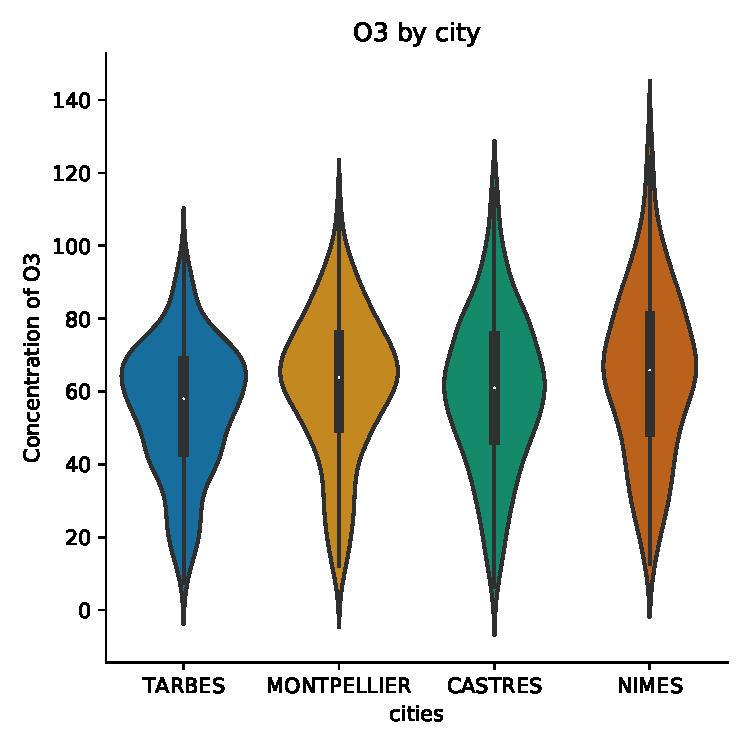
\includegraphics[width=\textwidth]{O3_by_city.pdf}
\caption{Violin plot to compare the concentration of ozone between four cities in Occitanie.}
    \label{fig:f1}
  \end{subfigure}
  \hfill
  \begin{subfigure}[b]{0.49\textwidth}
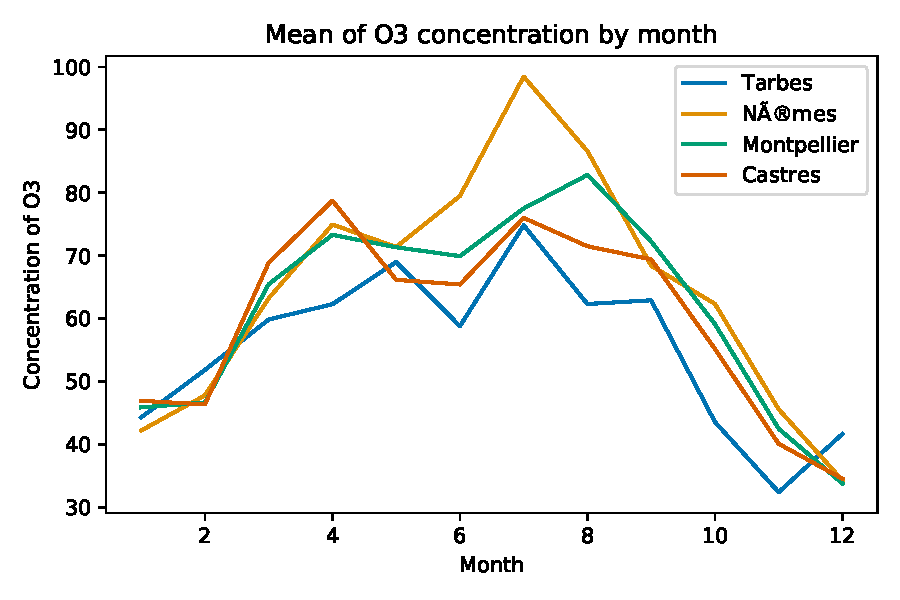
\includegraphics[width=\textwidth]{Mean_of_O3.pdf}
\vspace{.35cm}
\caption{Mean of O3 by month for four cities.}
    \label{fig:f2}
  \end{subfigure}
\end{figure}

\end{frame}


%%%%%%%%%%%%%%%%%%%%%%%%%%%%%%%%%%%%%%%%%%%%%%%%%%%%%%%%%%%%%%%%%%%%%%%%%%%%%%
%%%%%%%%%%%%%%%%%%%%%%%     ANOVA model     %%%%%%%%%%%%%%%%%%%%%%%%%%%%%%%%%%
%%%%%%%%%%%%%%%%%%%%%%%%%%%%%%%%%%%%%%%%%%%%%%%%%%%%%%%%%%%%%%%%%%%%%%%%%%%%%

\begin{frame}{Statistical model}
\begin{alertblock}{Model equation}
\[y_{ij}=\mu_i^*+\varepsilon_{ij}\]
\end{alertblock}

\medskip

 \begin{itemize}
        \item $\varepsilon_{ij} \overset{\iid}{\sim} \mathcal{N}(0,\sigma^2) $ is the noise
and $\cov(\epsilon_{ij},\varepsilon_{i'j'})=\sigma^2 \delta_{ii'} \delta_{jj'} $
        \item $y_{ij}$ is the $j^{th}$ measure for the modality
        \item $\bar{y}_n$ is the average of $y$ \ie
    \end{itemize}
 \[
\bar{y}_n= \frac{1}{n} \sum_{i=1}^I \sum_{j=1}^{n_i}y_{ij} ; i\in \llbracket 1,I \rrbracket. \]

\begin{onlyenv}<2>
\begin{itemize}
    \item  We sometimes  write : $\mu^*_i=\mu^*+\alpha^*_i $ to show the global mean effect and the specific effect of each feature.
\end{itemize}
\end{onlyenv}

\end{frame}

%%%%%%%%%%%%%%%%%%%%%%%%%%%%%%%%%%%%%%%%%%%%%%%%%%%%%%%%%%%%%%%%%%%%%%%%%%%%%%%
%%%%%%%%%%%%%%%%%%%%%%      ANOVA  results and normality assumption                   %%%%%%%%%%%%%%%%%%%%%%
%%%%%%%%%%%%%%%%%%%%%%%%%%%%%%%%%%%%%%%%%%%%%%%%%%%%%%%%%%%%%%%%%%%%%%%%%%%%%%%

\begin{Framecode}{Results from ANOVA and normality hypothesis}

\begin{verbatim}
poll = ols('valeur_originale ~ C(nom_com)',data=df).fit()
sm.stats.anova_lm(poll, typ=2) 
_, (__, ___, r) = sp.stats.probplot(poll.resid, fit=True)
\end{verbatim}

\begin{columns}
\begin{column}[T]{.55\textwidth}
 \vspace{.5cm}
\begin{table}
\caption{Results from the ANOVA on the $O_3$ concentration by cities.}
\setlength{\tabcolsep}{0.7\tabcolsep}
\begin{tabular}{|c|c|c|c|c|}
\hline
 &  sum\_sq      &  df    &  PR(>F) \\
    \small{C(nom\_com)} &  $16471.58$    & $3$  & $3.86e^{-08}$ \\
    \hline
\end{tabular}
\end{table}


\end{column}
\begin{column}[T]{.44\textwidth}

\begin{figure}
    \centering
    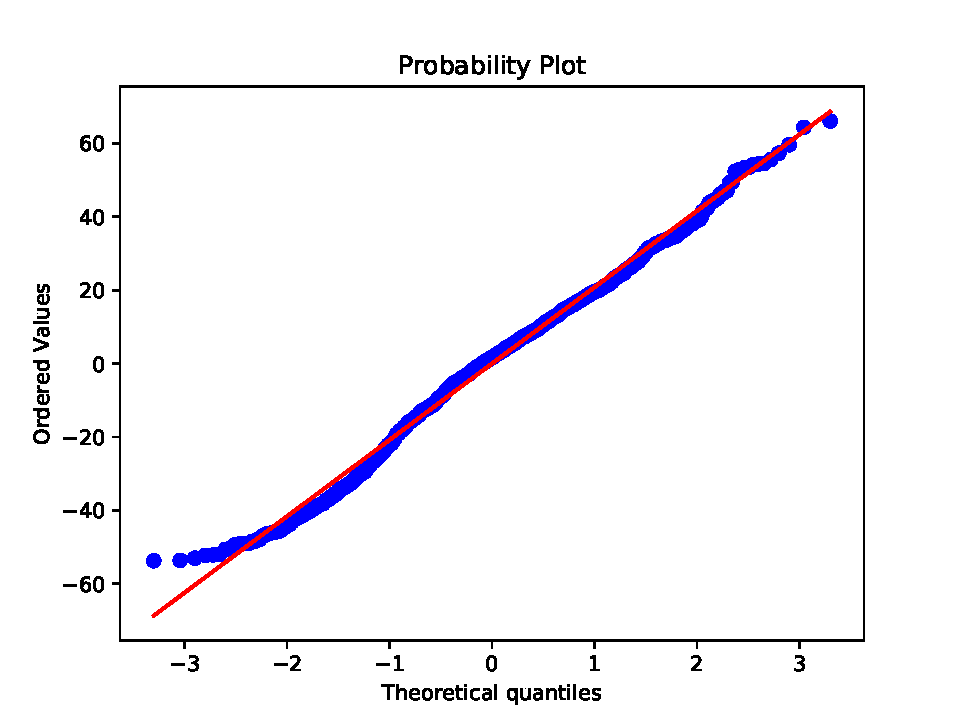
\includegraphics[width=\textwidth]{Verification_of_residues.pdf}
    \caption{Check residues normality assumption}
    \label{fig:check_res}
\end{figure}
\end{column}
\end{columns}    
\end{Framecode}

%%%%%%%%%%%%%%%%%%%%%%%%%%%%%%%%%%%%%%%%%%%%%%%%%%%%%%%%%%%%%%%%%%%%%%%%%%%%%%%
%%%%%%%%%%%%%%%%     Estimators in  ANOVA      %%%%%%%%%%%%%%%%%%%%%%
%%%%%%%%%%%%%%%%%%%%%%%%%%%%%%%%%%%%%%%%%%%%%%%%%%%%%%%%%%%%%%%%%%%%%%%%%%%%%%%
\begin{frame}
\rem
If we have an estimator for $\mu^*$ and $\alpha_i^*$ for all $i=1,\dots I$, noted $\hat{\mu}$ and $\hat{\alpha}$ : 

\[\hat{\mu}_i=  \hat{\mu} +  \hat{\alpha_i}  \]

and 

\begin{equation}\label{eq:sep}
(\hat{\mu}_1, \dots, \hat{\mu}_I) \in \argmin_{(\mu_1,\dots,\mu_I)\in \mathbb{R}^I} \frac{1}{2} \sum_{i=1}^I \sum_{j=1}^{n_i}(y_{ij}-\mu_i)^2
\end{equation}

\visible<2->{
\begin{alertblock}{}
Thanks to the separability principle:
\[\min_{(x_1,\dots,x_d)}f(x_1,\dots,x_d) \Longleftrightarrow \min_{x_j} g_j(x_j), \ j=1,\dots,d. \]

we have
\[\hat{\mu}_i=\frac{1}{n_i} \sum_{j=1}^{n_i}y_{ij} = \bar{y}_{i,:}.\]
\end{alertblock}
}
\end{frame}


%%%%%%%%%%%%%%%%%%%%%%%%%%%%%%%%%%%%%%%%%%%%%%%%%%%%%%%%%%%%%%%%%%%%%%%%%%%%%%%
%%%%%%%%%%%%%%%%%%%%%%      ANOVA  with the constraint sum of alpha i=0                   %%%%%%%%%%%%%%%%%%%%%%
%%%%%%%%%%%%%%%%%%%%%%%%%%%%%%%%%%%%%%%%%%%%%%%%%%%%%%%%%%%%%%%%%%%%%%%%%%%%%%%

\section{ANOVA with the constraint $\sum\alpha^*_i=0$}

\begin{frame}{ANOVA : case of a modeling with  : $\sum\alpha^*_i=0$}

Notice that if we change $\mu^*\longrightarrow \mu^*+\delta$ and $\alpha^*_i\longrightarrow \alpha^*_i-\delta$ then : $\mu_i^*=(\mu^* + \delta)+(\alpha_i^*-\delta)$

\begin{itemize}\setlength{\itemsep}{5pt}
\visible<1->{\item  \textbf{hypothesis} : $\sum\limits_{i=1}^{I}\alpha_i^*=0 $ \ie $\alpha_I^*=-\sum\limits_{i=1}^{I-1}\alpha_i^*$\\}
\visible<2->{\item \textbf{associated estimator} : $$\argmin\limits_{(\mu,\alpha)\in \mathbb{R} \times \mathbb{R}^I} \frac{1}{2} \sum\limits_{i=1}^I \sum\limits_{j=1}^{n_1}(y_{ij}-\mu - \alpha_i)^2$$}
\visible<3->{\item \textbf{Lagrangian} : $$\mathcal{L}(\mu,\alpha,\lambda)=\frac{1}{2} \sum\limits_{i=1}^I \sum\limits_{j=1}^{n_i}(y_{ij}-\mu - \alpha_i)^2 + \lambda \sum\limits_{i=1}^{I}\alpha_i $$}
\end{itemize}

\end{frame}

%%%%%%%%%%%%%%%%%%%%%%%%%%%%%%%%%%%%%%%%%%%%%%%%%%%%%%%%%%%%%%%%%%%%%%%%%%%%%%%
%%%%%%%%%%%%%%%%%%%%%%    Resolution of the optimization system                %%%%%%%%%%%%%%%%%%%%%%
%%%%%%%%%%%%%%%%%%%%%%%%%%%%%%%%%%%%%%%%%%%%%%%%%%%%%%%%%%%%%%%%%%%%%%%%%%%%%%%
\begin{frame}{Resolution of the optimization system}
\[\nabla \mathcal{L}(\hat\mu,\hat\alpha,\hat\lambda)=0\]

\[
\begin{aligned}
\begin{cases}
\sum\limits_{i=1}^{I}\hat{\alpha}_i=0 \\
\frac{\partial \mathcal{L}}{\partial \hat\mu}=0\\
\frac{\partial \mathcal{L}}{\partial \hat\alpha_{i_0}}=0\ \forall i_0
\end{cases}
\quad&\Longleftrightarrow\quad
\begin{cases}
\sum\limits_{i=1}^{I}\hat{\alpha_i}=0 \\
n\hat{\mu}+ \sum\limits_{i=1}^I n_i\hat{\alpha_i}-n\bar{y}_n=0\\
n_{i_0} \hat{\mu} +n_{i_0} \hat{\alpha_{i_0}} = n_{i_0}\bar{y}_{i_0,:} - \hat\lambda
\end{cases} \\
& \Longleftrightarrow\quad
\begin{cases}
\displaystyle\sum_{i=1}^{I}\hat{\alpha}_i=0  \\
\hat{\mu}+\frac{1}{n} \sum\limits_{i=1}^I n_i \hat{\alpha}_i=\bar{y}_n \\
n_{i_0}(\hat{\mu}+\hat{\alpha}_{i_0}-\bar{y}_{i_0,:}) +\hat{\lambda}=0 
\end{cases}
\end{aligned}
\]

\end{frame}

%%%%%%%%%%%%%%%%%%%%%%%%%%%%%%%%%%%%%%%%%%%%%%%%%%%%%%%%%%%%%%%%%%%%%%%%%%%%%%%
%%%%%%%%%%%%%%%%%%%%%%    Resolution of the optimization system   continuity              %%%%%%%%%%%%%%%%%%%%%%
%%%%%%%%%%%%%%%%%%%%%%%%%%%%%%%%%%%%%%%%%%%%%%%%%%%%%%%%%%%%%%%%%%%%%%%%%%%%%%%

\begin{frame}{Resolution of the optimization system}

\vspace{0.5cm}
We have :  
$\sum\limits_{i_0 =1}^{I} n_{i_0}(\hat{\mu}+\hat{\alpha}_{i_0}-\bar{y}_{i_0,:}) +I\hat{\lambda}=0$, so for $i_0=1,\cdots,I$, so we get

\visible<2->{
\[
\begin{aligned}
& \sum_{i_0=1}^{I}n_{i_0}(\hat{\mu}+\hat{\alpha}_{i_0}-\bar{y}_{i_0}) + I\hat{\lambda}=0 \\
\Longleftrightarrow\quad & n\hat{\mu}+ \sum\limits_{i_0=1}^{I} n_{i_0}\hat{\alpha}_{i_0}- \sum\limits_{i_0=1}^{I} n_{i_0}\bar{y}_{i_0,:}+I\hat{\lambda}=0 \\
\Longleftrightarrow\quad & n\hat{\mu}+ \sum\limits_{i_0=1}^{I} n_{i_0}\hat{\alpha}_{i_0}- n\bar{y}_n+I\hat{\lambda}=0  \\
\Longleftrightarrow\quad & I\hat{\lambda}=0 \Leftrightarrow \hat{\lambda}=0 
\end{aligned}
\]}

\end{frame}


%%%%%%%%%%%%%%%%%%%%%%%%%%%%%%%%%%%%%%%%%%%%%%%%%%%%%%%%%%%%%%%%%%%%%%%%%%%%%%%
%%%%%%%%%%%%%%%%%%%%%%    Results of the optimization system                %%%%%%%%%%%%%%%%%%%%%%
%%%%%%%%%%%%%%%%%%%%%%%%%%%%%%%%%%%%%%%%%%%%%%%%%%%%%%%%%%%%%%%%%%%%%%%%%%%%%%%


\begin{frame}

\begin{alertblock}{Results: }
    \begin{itemize}
        \item $\hat{\alpha}_{i_0} + \hat{\mu}= \bar{y}_{i_0,:}$
        \item $\hat{\mu}=\dfrac{1}{I}\sum\limits_{i_0=1}^{I} \bar{y}_{i_0,:}$
    \end{itemize}

Meaning that 
\[\hat{\alpha}_{i_0}=\bar{y}_{i_0,:}-\frac{1}{I} \sum\limits_{i_0=1}^{I} \bar{y}_{i_0,:}.\]

\end{alertblock}

\begin{alertblock}{Notice: }
    \begin{itemize}
        \item $ \hat{\mu} \ne \frac{1}{n}\sum\limits_{i=1}^{I}\sum\limits_{j=1}^{n_i}y_{ij}=\bar{y}_n$
        \item It might be different if there are $ i,i'$ such that: $n_i \ne n_{i'}$
    \end{itemize}


\end{alertblock}
\end{frame}

%%%%%%%%%%%%%%%%%%%%%%%%%%%%%%%%%%%%%%%%%%%%%%%%%%%%%%%%%%%%%%%%%%%%%%%%%%%%%%%
%%%%%%%%%%%%%%%%%%%%%%     ANOVA  with the constraint sum of n i alpha i=0             %%%%%%%%%%%%%%%%%%%%%%
%%%%%%%%%%%%%%%%%%%%%%%%%%%%%%%%%%%%%%%%%%%%%%%%%%%%%%%%%%%%%%%%%%%%%%%%%%%%%%%


\section{ANOVA with the constraint $\sum\limits_{i=1}^I n_i \alpha_i=0$}
\begin{frame}{The weighted sum of the individual effects is zero}

    \begin{itemize}
        \item  \textbf{hypothesis} : \[\sum_{i=1}^{I}n_i \alpha_i=0\]\\
         
        \item \textbf{associated estimator} : \[\argmin\limits_{(\mu,\alpha)\in \mathbb{R} \times \mathbb{R}^I} \frac{1}{2} \sum_{i=1}^I \sum_{j=1}^{n_i}(y_{ij}-\mu - \alpha_i)^2\]
        \item \textbf{Lagrangian} : \[\mathcal{L}(\mu,\alpha,\lambda)=\frac{1}{2} \sum_{i=1}^I \sum_{j=1}^{n_i}(y_{ij}-\mu - \alpha_i)^2 + \lambda \sum_{i=1}^{I}n_i\alpha_i \]
    \end{itemize}



\end{frame}

%%%%%%%%%%%%%%%%%%%%%%%%%%%%%%%%%%%%%%%%%%%%%%%%%%%%%%%%%%%%%%%%%%%%%%%%%%%%%%%
%%%%%%%%%%%%%%%%%%%%%%    Resolution of the optimization system                %%%%%%%%%%%%%%%%%%%%%%
%%%%%%%%%%%%%%%%%%%%%%%%%%%%%%%%%%%%%%%%%%%%%%%%%%%%%%%%%%%%%%%%%%%%%%%%%%%%%%%

\begin{frame}{Resolution of the optimization system}
\[\nabla \mathcal{L}(\hat\mu,\hat\alpha,\hat\lambda)=0\]
\[
\begin{aligned}
\begin{cases}
&  \sum\limits_{i=1}^{I}n_i \hat{\alpha}_i=0 \\
&  \frac{\partial \mathcal{L}}{\partial \mu}=0 \\
&  \frac{\partial \mathcal{L}}{\partial \alpha_{i_0}}=0\ \forall i_0 
\end{cases}
\quad&\Longleftrightarrow\quad
\begin{cases}
&  \sum\limits_{i=1}^{I}n_i\hat{\alpha}_i=0 \\
&  n\hat{\mu}+ \sum\limits_{i=1}^I n_i\hat{\alpha}_i-n\bar{y}_n=0 \\
&  \hat{\mu}+\hat{\alpha}_{i_0}-\bar{y}_{i_0,:}+\hat{\lambda} = 0, \forall{i_0} 
\end{cases}\\
& \Longleftrightarrow\quad
\begin{cases}
& \sum\limits_{i=1}^{I}n_i \hat{\alpha}_i=0 \\
& \hat{\mu}=\bar{y}_n \\
& \hat{\alpha}_{i_0} = \bar{y}_{i_0,:}-\hat{\lambda}-\bar{y}_n, \forall i_0

\end{cases}
\end{aligned}
\]

\end{frame}

%%%%%%%%%%%%%%%%%%%%%%%%%%%%%%%%%%%%%%%%%%%%%%%%%%%%%%%%%%%%%%%%%%%%%%%%%%%%%%%
%%%%%%%%%%%%%%%%%%%%%%    Results of the optimization system                %%%%%%%%%%%%%%%%%%%%%%
%%%%%%%%%%%%%%%%%%%%%%%%%%%%%%%%%%%%%%%%%%%%%%%%%%%%%%%%%%%%%%%%%%%%%%%%%%%%%%%

\begin{frame}

\begin{alertblock}{Results : }
    \begin{itemize}
        \item We multiply the third line of the equation by $n_{i_0}$ then we add them up for $i_0$ in $1$ to $I$. We finally obtain $\hat{\lambda}=0$, 
        \item $\hat{\mu}=\bar{y}_n$
    \end{itemize}
Meaning that:
\[\hat{\alpha}_{i_0}=\bar{y}_{i_0,:}- \bar{y}_{n}.\]
\end{alertblock}


\begin{alertblock}{Notice : }

The next case to study will be: $$ \alpha_{i_0}=0$$

\end{alertblock}

\end{frame}

\section{Non parametric alternative: permutation test}

%%%%%%%%%%%%%%%%%%%%%%%%%%%%%%%%%%%%%%%%%%%%%%%%%%%%%%%%%%%%%%%%%%%%%%%%%%%%%
%%%%%%%%%%%%%%%%%%%%%%%%%%    Permutation test   %%%%%%%%%%%%%%%%%%%%%%%%%%%%%%%%
%%%%%%%%%%%%%%%%%%%%%%%%%%%%%%%%%%%%%%%%%%%%%%%%%%%%%%%%%%%%%%%%%%%%%%%%%%%%%

\begin{frame}{Permutation test: medical scenario}
\begin{columns}
\begin{column}[T]{.48\textwidth}

\textbf{Protocol (Monte-Carlo):}
\begin{itemize}
    \visible<1->{\item $2$ groups: A the control and B the test, we test the effect of the treatment,}
    \visible<2->{\item $H0$: $\mu_A^* \geq \mu_B^*$ (Test if the treatment is better),}
    \visible<3->{\item Assign values for the effect of the treatment,}
    \visible<4->{\item Get the reference statistic: $\hat\mu_B - \hat\mu_A$,}
    \visible<5->{\item shuffle the groups and recalculate the test statistic $J$ times,}
    \visible<6->{\item $p$-value is the number of statistics over the reference divided by $J$.}

\end{itemize}
\end{column}
\begin{column}[T]{.48\textwidth}
\vspace{-.35cm}
	\begin{figure}[!tbp]
    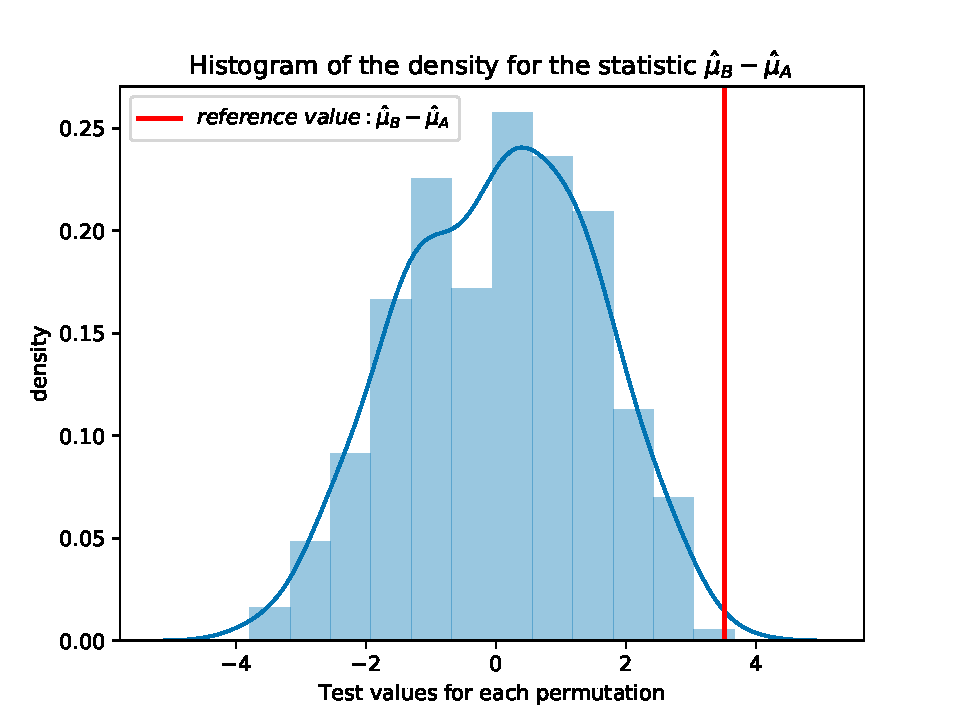
\includegraphics[width=\textwidth, clip, trim={0cm 0.2cm 0cm .5cm}]{rejet.pdf}
    \caption{\tiny{$\mu_A^*=3,\ \mu_B^*=7$, we reject the equality.}}
\end{figure}
\vspace{-.45cm}
\begin{figure}
    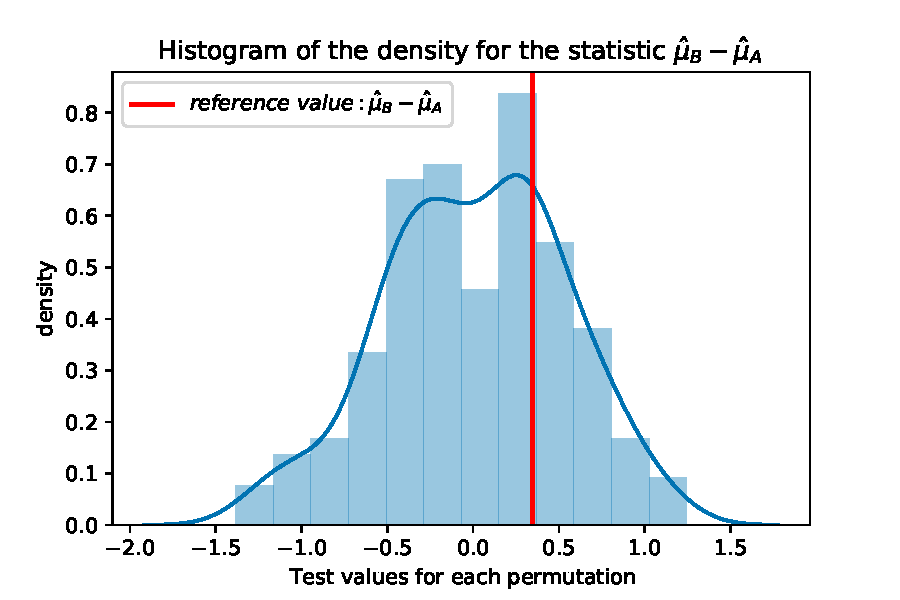
\includegraphics[width=\textwidth, clip, trim={0cm 0.2cm 0cm .5cm}]{not_rejet.pdf}
    \caption{\tiny{$\mu_A^*=2, \ \mu_B^*=2.5$, we don't reject the equality.}}
\end{figure}
	
\end{column}
\end{columns}
\end{frame}

\begin{frame}{Case: $\alpha_{i_0}=0$}

Our 3 hypotheses:

\begin{itemize}
    \item $\sum\limits_{i=1}^{I}\alpha_u=0$
    
    \item $\sum\limits_{i=1}^{I}\alpha_ix_i=0$
    
    \item $\alpha_{i_0}=0$
\end{itemize}

\begin{onlyenv}<2>

Associated estimator:


\[\min_{(\mu,\alpha)\in\mathbb{R}\times\mathbb{R}^I}\frac{1}{2}\sum\limits_{i=1}^{I}\sum\limits_{j=1}^{n}(\mu+\alpha_i-y_{i,j})^2\]
\[\mathcal{L}(\mu,\alpha,\lambda)=\sum\limits_{i=1}^{I}\sum\limits_{j=1}^{n}(\mu+\alpha_i-y_{i,j})^2+\lambda\alpha_{i_0}\]

\end{onlyenv}
\end{frame}

\begin{frame}{Case: $\alpha_{i_0}=0$}
\begin{itemize}
    \item $i\ne i_0: \frac{\partial\mathcal{L}}{\partial\alpha_i}=\sum\limits_{i=1}^{n_i}[\hat{\mu}+\hat{\alpha_i}-y_{i,j}]=0\;\;\; (*)$
    \item $i=i_0: \frac{\partial\mathcal{L}}{\partial\alpha_{i_0}}=\sum\limits_{i=1}^{n_i}[\hat{\mu}+\hat{\alpha_i}-y_{i,j}]+\hat{\lambda}=0\;\;\; (**)$
    \item $\hat{\mu}=y_{i_0,j}-\hat{\lambda}$
\end{itemize} 
\end{frame}

\begin{frame}{Case: $\alpha_{i_0}=0$}
\begin{aligned}
\sum\limits_{i\ne i_0}(*)+(**)&=\sum\limits_{i\ne i_0}\sum\limits_{j=1}^{n_{i_0}}\hat{\mu}+\sum\limits_{j=1}^{n_{i_0}}\hat{\mu}+\sum\limits_{i\ne i_0}\hat{\alpha_i}+n_{i_0}\hat{\alpha}_{i_0}-\sum\limits_{i\ne i_0}\sum\limits_{j}y_{i,j}\\
&-\sum\limits_{j=1}^{n_{i_0}}y_{i,j}\\
&= \sum\limits_{i}\sum\limits_{j}\hat{\mu} +\sum\limits_{i}n_i\hat{\alpha_i}-\sum\limits_{i}\sum\limits_{j}y_{i,j}+\hat{\lambda}\\
&=0
\end{aligned}
\end{frame}

\begin{frame}{Case: $\alpha_{i_0}=0$}
\[\sum\limits_{i\ne i_0}n_i\hat{\mu}+\sum\limits_{i\ne i_0}n_i\hat{\alpha}_i-\sum\limits_{i\ne i_0}\sum\limits_{j}y_{i,j}=0\]

With the previous equation:

\[n_{i_0}\hat{\mu}+n_{i_0}\hat{\alpha}_{i_0}-\sum\limits_{j=1}^{n_{i_0}}y_{i,j}+\hat{\lambda}=0\]

\begin{align*}
&\Longrightarrow \hat{\mu}+\hat{\alpha}_]{i_0}-\bar{y}_{i_0}+\frac{\hat{\lambda}}{n_{i_0}}\\
&\Longrightarrow \hat{\mu}=\bar{y}_{i,:}-\frac{\hat{\lambda}}{n_{i_0}}
\end{align*}
\end{frame}

\begin{frame}{Case: $\alpha_{i_0}=0$}
\begin{align*}
&n_i(\bar{y}_{i_0,:}-\frac{\hat{\lambda}}{n_{i_0}})+n_i\hat{\alpha}_i-n_i\bar{y}_{i,:}=0\\
&\Longrightarrow \hat{\alpha}_i=\frac{\hat{\lambda}}{n_{i_0}}-\bar{y_{i_0,:}+\bar{y_{i,:}}}
\end{align*}
We admit that $\hat{\lambda}=0$
\begin{align*}
    \Longrightarrow \begin{cases}
\hat{\alpha}_i=\bar{y}_{i,:}-\bar{y}_{i_0,:} \\
\hat{\alpha}_{i_0}=0\\
\hat{\mu}=\bar{y}_{i_0,:}\\
\frac{\partial \mathcal{L}}{\partial \hat\alpha_{i_0}}=0\ \forall i_0
\end{cases}
\end{align*}
\end{frame}

\begin{frame}{Variance estimator}
    \[\hat{\sigma}^2=\frac{1}{n-I}\sum\limits_{i=1}^{I}\sum\limits_{j=i}^{n_i}(\bar{y}_{i,:}-_{i,j})^2\]
    \begin{itemize}
        \item $n-I$: Correcton so that $\mathbb{E}(\hat{\sigma}^2)=\sigma^2$
        \item $y_{i,j}=\mu^{*}+\epsilon_{i,j}$
        \item $\epsilon_{i,j}\sim\mathcal{N}(0,\sigma^2)$ 
    \end{itemize}
\end{frame}

\begin{frame}{Variance estimator}
\begin{alertblock}{Notice : }
$X=[\mathbb{I}_{c_1},\dots,\mathbb{I}_{c_I}]\in \mathbb{R}^{n\times I}$: 

\[\frac{1}{n-rg(X)} \|y-X\hat{\beta}^{LS}\|^2 \text{ unbiased estimator of } \sigma^2\]

$\sum\limits_{i=1}^{i}\mathbb{I}_{c_i}=\mathbb{I}_n$
$rg(\Tilde{X}=I,\Tilde{X}=[\mathbb{I}_n,\mathbb{I}_{c_n},\dots,\mathbb{I}_{c_I}]$
\end{alertblock}
\end{frame}

\begin{frame}{Test: "are the terms different"}
\begin{alertblock}{Our $H_0$}
$H_0:\mu_{1}^{*}=\mu_{2}^{*}=\dots=\mu_{I}^{*}$
\end{alertblock}
\begin{itemize}
    \item $F_{obs}=\frac{\frac{1}{I-1}\sum\limits_{i=1}^{I}(\bar{y}_{i,:}-\bar{y}_n)^2}{\hat{\sigma}^2}$ with: $F_{obs}\sim\Tilde{F}^{I-1}_{n-I}$
    \item We reject the test: $F_{obs}>F^{I-1}_{n-I}(1-\alpha)$ (if we want to test $\alpha$)
\end{itemize}

\end{frame}

\begin{frame}{Test: "are the terms different"}
\begin{alertblock}{Notice : }
For the test $\mu^{*}_{1}=\mu^{*}_{1}, we us the test of Student$
\end{alertblock}
\end{frame}

%%%%%%%%%%%%%%%%%%%%%%%%%%%%%%%%%%%%%%%%%%%%%%%%%%%%%%%%%%%%%%%%%%%%%%%%%%%%%
%%%%%%%%%%%%%%%%%%%%%%%%%%    Bibliography   %%%%%%%%%%%%%%%%%%%%%%%%%%%%%%%%
%%%%%%%%%%%%%%%%%%%%%%%%%%%%%%%%%%%%%%%%%%%%%%%%%%%%%%%%%%%%%%%%%%%%%%%%%%%%%

\begin{frame}{Bibliography}
\nocite{*}
\printbibliography
\end{frame}

\end{document}
